\section{Result}

\newcommand{\e}[1]{\times 10^{#1}}

The frequency we read from the signal generator is $f=34498 \pm 1$Hz. The
temperature is $23 \pm 1 ^\circ C$.

\subsection{Measurements for resonance method}

The measurements are shown in Table~\ref{data_res} with the calculation for $L_{10+i}-L_i$.


\begin{table}[H] \small
    \centering
    \begin{tabular}{|c|c|c|c|c|c|}
    \hline
        \multicolumn{2}{|c|}{$L_i[\times 10^{-3} m]\pm[0.01\times 10^{-3} m]$} & 
        \multicolumn{2}{|c|}{$L_i[\times 10^{-3} m]\pm[\times 10^{-3} m]$} &
        \multicolumn{2}{|c|}{$L_{10+i}-L_i[\e{-3}m]$}\\\hline
        1  & 29.37 & 11 &  80.44 & 1  & 51.07 \\\hline
        2  & 34.49 & 12 &  85.48 & 2  & 50.99 \\\hline
        3  & 39.60 & 13 &  90.01 & 3  & 50.41 \\\hline
        4  & 44.74 & 14 &  95.65 & 4  & 50.91 \\\hline
        5  & 49.83 & 15 & 100.82 & 5  & 50.99 \\\hline
        6  & 54.90 & 16 & 105.93 & 6  & 51.03 \\\hline
        7  & 60.06 & 17 & 111.12 & 7  & 51.06 \\\hline
        8  & 65.24 & 18 & 116.20 & 8  & 50.96 \\\hline
        9  & 70.37 & 19 & 121.32 & 9  & 50.95 \\\hline
        10 & 75.38 & 20 & 126.39 & 10 & 51.01 \\\hline
    \end{tabular}
    \caption{Data for the resonance method}\label{data_res}
\end{table}

The average value of $\Delta L$ is calculated  based on the results presented in Table \ref{data_res} as

\[
    \overline{\Delta L}=\frac{1}{10}\sum_{i=1}^{10}\Delta L_i=(50.94\pm 0.05)\times 10^{-3} m,\quad u_{r,\Delta}=0.10\%.
\]

Hence, the wavelength $\lambda$ can be calculated as

\[
        \lambda=\frac{2\Delta L}{n}=\frac{2\times50.94\times 10^{-3} }{10}=(10.19 \pm0.01)\times 10^{-3} m,\quad u_{r,\lambda}=0.10\%.
\]

The speed of sound in air $v$ is

\[
    v=\lambda f = (10.19 \pm 0.01)\times 10^{-3} m \cdot 34498 Hz  = 351.45 \pm 0.4 m/s,\quad u_{r,v}=0.11\%.
\]

\subsection{Measurements for phase comparison method}

The measurements are shown in Table~\ref{data_pha} with the calculation for $L_{6+i}-L_i$.

\begin{table}[H] \small
    \centering
    \begin{tabular}{|c|c|c|c|c|c|}
    \hline
        \multicolumn{2}{|c|}{$L_i[\times 10^{-3} m]\pm[0.01\times 10^{-3} m]$} & 
        \multicolumn{2}{|c|}{$L_i[\times 10^{-3} m]\pm[0.01\times 10^{-3} m]$} &
        \multicolumn{2}{|c|}{$L_{6+i}-L_i[\e{-3}m]$}\\\hline
        1 & 23.57 & 7  &  84.39 & 1 & 60.82 \\\hline
        2 & 33.78 & 8  &  94.51 & 2 & 60.73 \\\hline
        3 & 43.97 & 9  & 104.62 & 3 & 60.65 \\\hline
        4 & 54.17 & 10 & 114.76 & 4 & 60.59 \\\hline
        5 & 64.11 & 11 & 124.72 & 5 & 60.61 \\\hline
        6 & 74.24 & 12 & 134.92 & 6 & 60.68 \\\hline
    \end{tabular}
    \caption{Data for the phase comparison method}\label{data_pha}
\end{table}
    
The average value of $\Delta L$ is calculated  based on the results presented in Table \ref{data_res} as

\[
    \overline{\Delta L}=\frac{1}{6}\sum_{i=1}^{6}\Delta L_i=(60.68\pm 0.8)\times 10^{-3} m,\quad u_{r,\Delta L}=3\%.
\]

Hence, the wavelength $\lambda$ can be calculated as

\[
    \lambda=\frac{\Delta L}{n}=\frac{60.68 \e{-3}}{6}=(10.11 \pm 0.13)\times 10^{-3} m,\quad u_{r,\lambda}=1.3\%.
\]

The speed of sound in air $v$ is

\[
    v=\lambda f = (10.11 \pm 0.13) \times 10^{-3} m \cdot 34498 Hz  = 348.889 \pm 0.4 m/s,\quad u_{r,v}=0.11\%.
\]

\subsection{Measurements for time difference method (liquid)}

We obtain the speed of sound in water from Table \ref{data_tim} by linear fitting (See Figure \ref{lt}).
    
\begin{table}[H] \small
    \centering
    \begin{tabular}{|c|c|c|}
    \hline
        & $t_i[\e{-6}s] \pm 0.2 [\e{-6} s]$  & $L_i[\times 10^{-3} m] \pm 0.01 [\e{-3} m]$ \\\hline
        1  & 113.8 & 160.00 \\\hline
        2  & 120.6 & 170.00 \\\hline
        3  & 127.4 & 180.00 \\\hline
        4  & 134.2 & 190.00 \\\hline
        5  & 141.2 & 200.00 \\\hline
        6  & 148.2 & 210.00 \\\hline
        7  & 153.8 & 220.00 \\\hline
        8  & 160.6 & 230.00 \\\hline
        9  & 167.4 & 240.00 \\\hline
        10 & 174.2 & 250.00 \\\hline
        11 & 181.0 & 260.00 \\\hline
        12 & 186.8 & 270.00 \\\hline
    \end{tabular}
    \caption{Data for Figure \ref{lt}}\label{data_tim}
\end{table}
\begin{figure}[H]
    \centering
    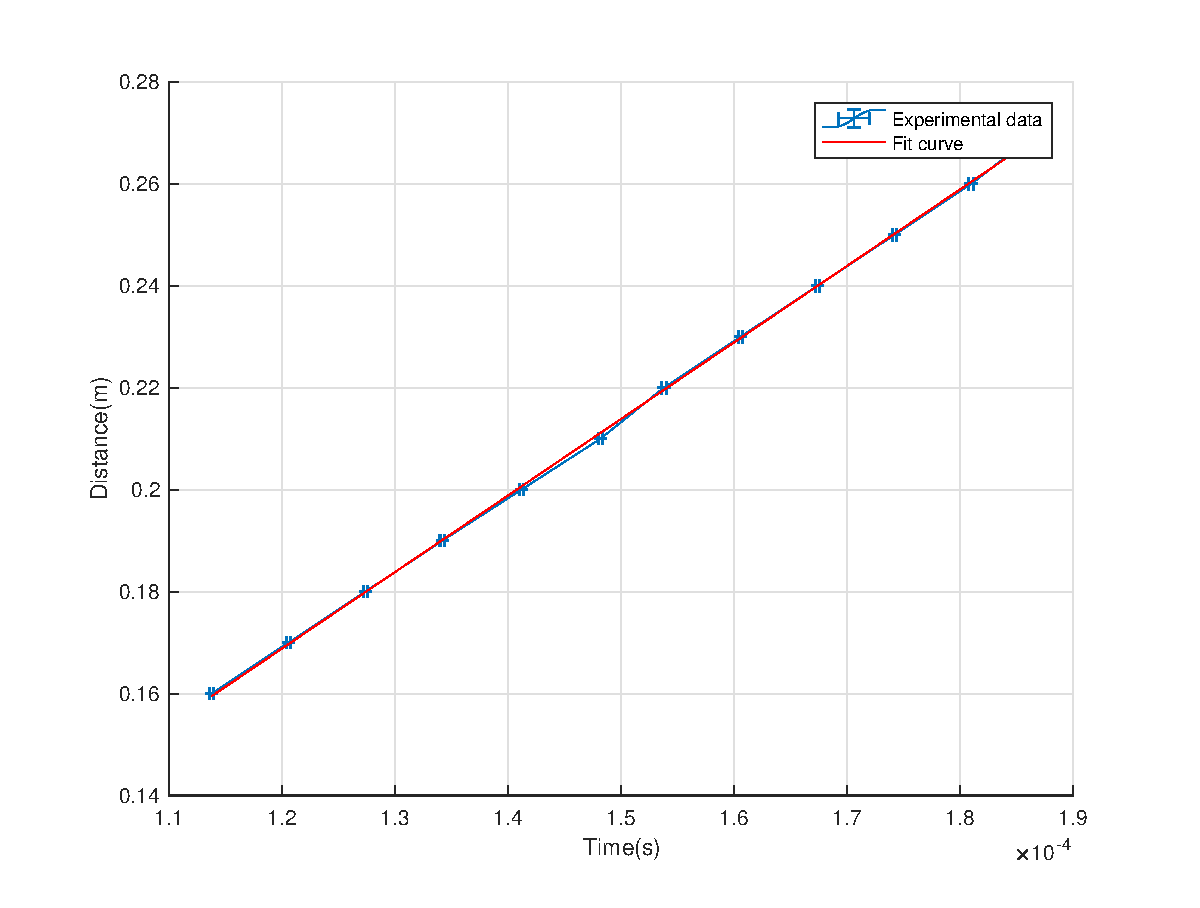
\includegraphics[width=12cm]{fig/tl}
    \caption{Fitting curve for $L\ vs.\ t$. }\label{lt}
\end{figure}

\begin{quote}
Goodness of fit:\\
  SSE: 3.331e-06                \\
  R-square: 0.9998              \\
  Adjusted R-square: 0.9997     \\
  RMSE: 0.0005771               
\end{quote}

From the data processing of Matalb we know about the slope that 
\[
    v_{water}=1502 \pm 16 m/s.
\]